% Options for packages loaded elsewhere
\PassOptionsToPackage{unicode}{hyperref}
\PassOptionsToPackage{hyphens}{url}
%
\documentclass[
]{article}
\usepackage{amsmath,amssymb}
\usepackage{lmodern}
\usepackage{ifxetex,ifluatex}
\ifnum 0\ifxetex 1\fi\ifluatex 1\fi=0 % if pdftex
  \usepackage[T1]{fontenc}
  \usepackage[utf8]{inputenc}
  \usepackage{textcomp} % provide euro and other symbols
\else % if luatex or xetex
  \usepackage{unicode-math}
  \defaultfontfeatures{Scale=MatchLowercase}
  \defaultfontfeatures[\rmfamily]{Ligatures=TeX,Scale=1}
\fi
% Use upquote if available, for straight quotes in verbatim environments
\IfFileExists{upquote.sty}{\usepackage{upquote}}{}
\IfFileExists{microtype.sty}{% use microtype if available
  \usepackage[]{microtype}
  \UseMicrotypeSet[protrusion]{basicmath} % disable protrusion for tt fonts
}{}
\makeatletter
\@ifundefined{KOMAClassName}{% if non-KOMA class
  \IfFileExists{parskip.sty}{%
    \usepackage{parskip}
  }{% else
    \setlength{\parindent}{0pt}
    \setlength{\parskip}{6pt plus 2pt minus 1pt}}
}{% if KOMA class
  \KOMAoptions{parskip=half}}
\makeatother
\usepackage{xcolor}
\IfFileExists{xurl.sty}{\usepackage{xurl}}{} % add URL line breaks if available
\IfFileExists{bookmark.sty}{\usepackage{bookmark}}{\usepackage{hyperref}}
\hypersetup{
  pdftitle={HW 8\_Onyango},
  pdfauthor={Brenda Onyango},
  hidelinks,
  pdfcreator={LaTeX via pandoc}}
\urlstyle{same} % disable monospaced font for URLs
\usepackage[margin=1in]{geometry}
\usepackage{color}
\usepackage{fancyvrb}
\newcommand{\VerbBar}{|}
\newcommand{\VERB}{\Verb[commandchars=\\\{\}]}
\DefineVerbatimEnvironment{Highlighting}{Verbatim}{commandchars=\\\{\}}
% Add ',fontsize=\small' for more characters per line
\usepackage{framed}
\definecolor{shadecolor}{RGB}{248,248,248}
\newenvironment{Shaded}{\begin{snugshade}}{\end{snugshade}}
\newcommand{\AlertTok}[1]{\textcolor[rgb]{0.94,0.16,0.16}{#1}}
\newcommand{\AnnotationTok}[1]{\textcolor[rgb]{0.56,0.35,0.01}{\textbf{\textit{#1}}}}
\newcommand{\AttributeTok}[1]{\textcolor[rgb]{0.77,0.63,0.00}{#1}}
\newcommand{\BaseNTok}[1]{\textcolor[rgb]{0.00,0.00,0.81}{#1}}
\newcommand{\BuiltInTok}[1]{#1}
\newcommand{\CharTok}[1]{\textcolor[rgb]{0.31,0.60,0.02}{#1}}
\newcommand{\CommentTok}[1]{\textcolor[rgb]{0.56,0.35,0.01}{\textit{#1}}}
\newcommand{\CommentVarTok}[1]{\textcolor[rgb]{0.56,0.35,0.01}{\textbf{\textit{#1}}}}
\newcommand{\ConstantTok}[1]{\textcolor[rgb]{0.00,0.00,0.00}{#1}}
\newcommand{\ControlFlowTok}[1]{\textcolor[rgb]{0.13,0.29,0.53}{\textbf{#1}}}
\newcommand{\DataTypeTok}[1]{\textcolor[rgb]{0.13,0.29,0.53}{#1}}
\newcommand{\DecValTok}[1]{\textcolor[rgb]{0.00,0.00,0.81}{#1}}
\newcommand{\DocumentationTok}[1]{\textcolor[rgb]{0.56,0.35,0.01}{\textbf{\textit{#1}}}}
\newcommand{\ErrorTok}[1]{\textcolor[rgb]{0.64,0.00,0.00}{\textbf{#1}}}
\newcommand{\ExtensionTok}[1]{#1}
\newcommand{\FloatTok}[1]{\textcolor[rgb]{0.00,0.00,0.81}{#1}}
\newcommand{\FunctionTok}[1]{\textcolor[rgb]{0.00,0.00,0.00}{#1}}
\newcommand{\ImportTok}[1]{#1}
\newcommand{\InformationTok}[1]{\textcolor[rgb]{0.56,0.35,0.01}{\textbf{\textit{#1}}}}
\newcommand{\KeywordTok}[1]{\textcolor[rgb]{0.13,0.29,0.53}{\textbf{#1}}}
\newcommand{\NormalTok}[1]{#1}
\newcommand{\OperatorTok}[1]{\textcolor[rgb]{0.81,0.36,0.00}{\textbf{#1}}}
\newcommand{\OtherTok}[1]{\textcolor[rgb]{0.56,0.35,0.01}{#1}}
\newcommand{\PreprocessorTok}[1]{\textcolor[rgb]{0.56,0.35,0.01}{\textit{#1}}}
\newcommand{\RegionMarkerTok}[1]{#1}
\newcommand{\SpecialCharTok}[1]{\textcolor[rgb]{0.00,0.00,0.00}{#1}}
\newcommand{\SpecialStringTok}[1]{\textcolor[rgb]{0.31,0.60,0.02}{#1}}
\newcommand{\StringTok}[1]{\textcolor[rgb]{0.31,0.60,0.02}{#1}}
\newcommand{\VariableTok}[1]{\textcolor[rgb]{0.00,0.00,0.00}{#1}}
\newcommand{\VerbatimStringTok}[1]{\textcolor[rgb]{0.31,0.60,0.02}{#1}}
\newcommand{\WarningTok}[1]{\textcolor[rgb]{0.56,0.35,0.01}{\textbf{\textit{#1}}}}
\usepackage{graphicx}
\makeatletter
\def\maxwidth{\ifdim\Gin@nat@width>\linewidth\linewidth\else\Gin@nat@width\fi}
\def\maxheight{\ifdim\Gin@nat@height>\textheight\textheight\else\Gin@nat@height\fi}
\makeatother
% Scale images if necessary, so that they will not overflow the page
% margins by default, and it is still possible to overwrite the defaults
% using explicit options in \includegraphics[width, height, ...]{}
\setkeys{Gin}{width=\maxwidth,height=\maxheight,keepaspectratio}
% Set default figure placement to htbp
\makeatletter
\def\fps@figure{htbp}
\makeatother
\setlength{\emergencystretch}{3em} % prevent overfull lines
\providecommand{\tightlist}{%
  \setlength{\itemsep}{0pt}\setlength{\parskip}{0pt}}
\setcounter{secnumdepth}{-\maxdimen} % remove section numbering
\ifluatex
  \usepackage{selnolig}  % disable illegal ligatures
\fi

\title{HW 8\_Onyango}
\author{Brenda Onyango}
\date{10/12/2021}

\begin{document}
\maketitle

\hypertarget{load-needed-packages}{%
\subsubsection{Load needed packages}\label{load-needed-packages}}

\begin{Shaded}
\begin{Highlighting}[]
\FunctionTok{library}\NormalTok{(tidyverse)}
\end{Highlighting}
\end{Shaded}

\begin{verbatim}
## -- Attaching packages --------------------------------------- tidyverse 1.3.1 --
\end{verbatim}

\begin{verbatim}
## v ggplot2 3.3.5     v purrr   0.3.4
## v tibble  3.1.5     v dplyr   1.0.7
## v tidyr   1.1.4     v stringr 1.4.0
## v readr   2.0.2     v forcats 0.5.1
\end{verbatim}

\begin{verbatim}
## -- Conflicts ------------------------------------------ tidyverse_conflicts() --
## x dplyr::filter() masks stats::filter()
## x dplyr::lag()    masks stats::lag()
\end{verbatim}

\begin{Shaded}
\begin{Highlighting}[]
\FunctionTok{library}\NormalTok{(janitor)}
\end{Highlighting}
\end{Shaded}

\begin{verbatim}
## 
## Attaching package: 'janitor'
\end{verbatim}

\begin{verbatim}
## The following objects are masked from 'package:stats':
## 
##     chisq.test, fisher.test
\end{verbatim}

\begin{Shaded}
\begin{Highlighting}[]
\FunctionTok{library}\NormalTok{(rstan)}
\end{Highlighting}
\end{Shaded}

\begin{verbatim}
## Loading required package: StanHeaders
\end{verbatim}

\begin{verbatim}
## rstan (Version 2.21.3, GitRev: 2e1f913d3ca3)
\end{verbatim}

\begin{verbatim}
## For execution on a local, multicore CPU with excess RAM we recommend calling
## options(mc.cores = parallel::detectCores()).
## To avoid recompilation of unchanged Stan programs, we recommend calling
## rstan_options(auto_write = TRUE)
\end{verbatim}

\begin{verbatim}
## 
## Attaching package: 'rstan'
\end{verbatim}

\begin{verbatim}
## The following object is masked from 'package:tidyr':
## 
##     extract
\end{verbatim}

\begin{Shaded}
\begin{Highlighting}[]
\FunctionTok{library}\NormalTok{(bayesplot)}
\end{Highlighting}
\end{Shaded}

\begin{verbatim}
## This is bayesplot version 1.8.1
\end{verbatim}

\begin{verbatim}
## - Online documentation and vignettes at mc-stan.org/bayesplot
\end{verbatim}

\begin{verbatim}
## - bayesplot theme set to bayesplot::theme_default()
\end{verbatim}

\begin{verbatim}
##    * Does _not_ affect other ggplot2 plots
\end{verbatim}

\begin{verbatim}
##    * See ?bayesplot_theme_set for details on theme setting
\end{verbatim}

\hypertarget{exercise-1}{%
\subsection{Exercise 1}\label{exercise-1}}

\begin{enumerate}
\def\labelenumi{\alph{enumi})}
\tightlist
\item
  The steps for grid approximation are:
\end{enumerate}

\begin{enumerate}
\def\labelenumi{\arabic{enumi})}
\tightlist
\item
  Define a discrete grid of possible theta values
\item
  evaluate the prior pdf of f(theta) and liklihood function
  L(theta\textbar y) at each theta grid value 3)Calculate the product of
  f(theta) * L(theta\textbar y) at each theta grid value and then
  normalize the products so they sum to 1
\item
  randomly sample N theta grid values
\end{enumerate}

\begin{enumerate}
\def\labelenumi{\alph{enumi})}
\setcounter{enumi}{1}
\tightlist
\item
  To make the approximation more accurate I would change the first step
  when defining a discrete grid. Increasing the number of grid values
  creates approximations that better match true posteriors.
\end{enumerate}

\hypertarget{exercise-2}{%
\subsection{Exercise 2}\label{exercise-2}}

\begin{Shaded}
\begin{Highlighting}[]
\CommentTok{\#Using code Yue shared to include picture}

\NormalTok{knitr}\SpecialCharTok{::}\FunctionTok{include\_graphics}\NormalTok{(}\StringTok{"/Users/brendaonyango/Desktop/IMG\_4318 copy.png"}\NormalTok{)}
\end{Highlighting}
\end{Shaded}

\includegraphics{/Users/brendaonyango/Desktop/IMG_4318 copy.png}

\hypertarget{exercise-3}{%
\subsection{Exercise 3}\label{exercise-3}}

\begin{enumerate}
\def\labelenumi{\alph{enumi})}
\item
  If the chain is mixing too slowly it will have only explored a limited
  range in the first several thousands iterations. It will overestimate
  the plausibility of pi values in this range and underestimate the
  plasuibility of values outside the range.
\item
  The chain having a high correlation will not estimate the correct
  peak, if there is one, in the posterior.
\item
  Chains that get stuck are overestimating in the values where they are
  stuck and will produce peaks in the posterior that are not there.
\end{enumerate}

\hypertarget{exercise-6.4}{%
\subsection{Exercise 6.4}\label{exercise-6.4}}

\begin{enumerate}
\def\labelenumi{\alph{enumi})}
\item
  MCMC diagnostics are important because simulations are not perfect and
  diagnostics, used holistically, can identify how to improve a MCMC
  chain.
\item
  MCMC simulations are helpful because they are an efficient and
  flexible alternative to grid approximations. Grid approximations for
  more complex problems take a long time and grid approximations are not
  good for estimating posteriors when there are multiple dimensions.
  MCMCs can.
\item
  Rstan combines R with the Stan ``engine''; Stan is written in C++ and
  is good for Bayesian modeling.
\item
  How to put Markov chains in applied language for social
  problems/questions.
\end{enumerate}

\hypertarget{exercise-6.5}{%
\subsection{Exercise 6.5}\label{exercise-6.5}}

We're given Y\textbar pi\textasciitilde Bin(n, pi) and
pi\textasciitilde Beta(3, 8) and n = 10 with Y = 2.

\begin{enumerate}
\def\labelenumi{\alph{enumi})}
\tightlist
\item
  Use grid approximation with values pi E\{0, 0.25, 0.50, .75,1\} to
  approximate posterior
\end{enumerate}

\begin{Shaded}
\begin{Highlighting}[]
\CommentTok{\#step 1: defining a grid with 5 pi values }
\NormalTok{grid\_data }\OtherTok{\textless{}{-}} \FunctionTok{data.frame}\NormalTok{(}\AttributeTok{pi\_grid =} \FunctionTok{seq}\NormalTok{(}\AttributeTok{from =} \DecValTok{0}\NormalTok{, }\AttributeTok{to =} \DecValTok{1}\NormalTok{, }\AttributeTok{length =} \DecValTok{5}\NormalTok{))}

\CommentTok{\# step 2: evaluating prior and liklihood at each pi}
\NormalTok{grid\_data }\OtherTok{\textless{}{-}}\NormalTok{ grid\_data }\SpecialCharTok{|}\ErrorTok{\textgreater{}} 
  \FunctionTok{mutate}\NormalTok{(}\AttributeTok{prior =} \FunctionTok{dbeta}\NormalTok{(pi\_grid, }\DecValTok{3}\NormalTok{,}\DecValTok{8}\NormalTok{), }
         \AttributeTok{liklihood =}\FunctionTok{dbinom}\NormalTok{(}\DecValTok{2}\NormalTok{,}\DecValTok{10}\NormalTok{, pi\_grid))}
\end{Highlighting}
\end{Shaded}

Next is approximating the posterior using the product of the liklihood
and prior and then normalizing them.

\begin{Shaded}
\begin{Highlighting}[]
\CommentTok{\#step 3: approximate the posterior}
\NormalTok{grid\_data }\OtherTok{\textless{}{-}}\NormalTok{ grid\_data }\SpecialCharTok{|}\ErrorTok{\textgreater{}} 
  \FunctionTok{mutate}\NormalTok{(}\AttributeTok{unnormalized =}\NormalTok{ liklihood }\SpecialCharTok{*}\NormalTok{ prior, }
         \AttributeTok{posterior =}\NormalTok{ unnormalized}\SpecialCharTok{/}\FunctionTok{sum}\NormalTok{(unnormalized))}

\CommentTok{\#confirming that posterior approximation sums to 1}
\NormalTok{grid\_data }\SpecialCharTok{|}\ErrorTok{\textgreater{}} \FunctionTok{summarize}\NormalTok{(}\FunctionTok{sum}\NormalTok{(unnormalized), }\FunctionTok{sum}\NormalTok{(posterior))}
\end{Highlighting}
\end{Shaded}

\begin{verbatim}
##   sum(unnormalized) sum(posterior)
## 1         0.8765603              1
\end{verbatim}

Next we'll examine the grid approxiation posterior rounded to 2 decimal
places.

\begin{Shaded}
\begin{Highlighting}[]
\CommentTok{\#step 4}
\FunctionTok{round}\NormalTok{(grid\_data, }\DecValTok{2}\NormalTok{) }\CommentTok{\#2 is indicating how many decimal points to use }
\end{Highlighting}
\end{Shaded}

\begin{verbatim}
##   pi_grid prior liklihood unnormalized posterior
## 1    0.00  0.00      0.00         0.00      0.00
## 2    0.25  3.00      0.28         0.85      0.96
## 3    0.50  0.70      0.04         0.03      0.04
## 4    0.75  0.01      0.00         0.00      0.00
## 5    1.00  0.00      0.00         0.00      0.00
\end{verbatim}

Finally, we'll plot this model.

\begin{Shaded}
\begin{Highlighting}[]
\CommentTok{\# plotting the grid approximation posterior}
\FunctionTok{ggplot}\NormalTok{(grid\_data, }\FunctionTok{aes}\NormalTok{(}\AttributeTok{x =}\NormalTok{ pi\_grid, }\AttributeTok{y =}\NormalTok{ posterior)) }\SpecialCharTok{+} 
  \FunctionTok{geom\_point}\NormalTok{() }\SpecialCharTok{+} 
  \FunctionTok{geom\_segment}\NormalTok{(}\FunctionTok{aes}\NormalTok{(}\AttributeTok{x =}\NormalTok{ pi\_grid, }\AttributeTok{xend =}\NormalTok{ pi\_grid, }\AttributeTok{y =} \DecValTok{0}\NormalTok{, }\AttributeTok{yend =}\NormalTok{ posterior))}
\end{Highlighting}
\end{Shaded}

\includegraphics{HW-8_files/figure-latex/unnamed-chunk-6-1.pdf}

\begin{enumerate}
\def\labelenumi{\alph{enumi})}
\setcounter{enumi}{1}
\tightlist
\item
  Now we're asked to repeat the above using a grid of 201 equally spaced
  values between 0 and 1.
\end{enumerate}

\begin{Shaded}
\begin{Highlighting}[]
\CommentTok{\#step 1}
\NormalTok{grd\_data }\OtherTok{\textless{}{-}} \FunctionTok{data.frame}\NormalTok{(}\AttributeTok{p\_grid =} \FunctionTok{seq}\NormalTok{(}\AttributeTok{from =} \DecValTok{0}\NormalTok{, }\AttributeTok{to =} \DecValTok{1}\NormalTok{, }\AttributeTok{length =} \DecValTok{201}\NormalTok{)) }\CommentTok{\#changed length to 201}

\CommentTok{\#step 2}
\NormalTok{grd\_data }\OtherTok{\textless{}{-}}\NormalTok{ grd\_data }\SpecialCharTok{|}\ErrorTok{\textgreater{}} \CommentTok{\#changed names of data, prior, liklihood to keep distinct from part a }
  \FunctionTok{mutate}\NormalTok{(}\AttributeTok{prir =} \FunctionTok{dbeta}\NormalTok{(p\_grid, }\DecValTok{3}\NormalTok{,}\DecValTok{8}\NormalTok{), }\CommentTok{\#prior remained the same }
         \AttributeTok{liklhood =} \FunctionTok{dbinom}\NormalTok{(}\DecValTok{2}\NormalTok{,}\DecValTok{10}\NormalTok{, p\_grid)) }\CommentTok{\#successes and outcomes remained teh same}
\CommentTok{\#step 3}
\NormalTok{grd\_data }\OtherTok{\textless{}{-}}\NormalTok{ grd\_data }\SpecialCharTok{|}\ErrorTok{\textgreater{}} 
  \FunctionTok{mutate}\NormalTok{(}\AttributeTok{unnormalized =}\NormalTok{ liklhood }\SpecialCharTok{*}\NormalTok{ prir, }
         \AttributeTok{posterir =}\NormalTok{ unnormalized}\SpecialCharTok{/}\FunctionTok{sum}\NormalTok{(unnormalized))}

\CommentTok{\#confirming that posterior approximation sums to 1}
\NormalTok{grd\_data }\SpecialCharTok{|}\ErrorTok{\textgreater{}} \FunctionTok{summarize}\NormalTok{(}\FunctionTok{sum}\NormalTok{(unnormalized), }\FunctionTok{sum}\NormalTok{(posterir))}
\end{Highlighting}
\end{Shaded}

\begin{verbatim}
##   sum(unnormalized) sum(posterir)
## 1          41.79567             1
\end{verbatim}

\begin{Shaded}
\begin{Highlighting}[]
\CommentTok{\#step 4}
\FunctionTok{round}\NormalTok{(grd\_data, }\DecValTok{2}\NormalTok{)}
\end{Highlighting}
\end{Shaded}

\begin{verbatim}
##     p_grid prir liklhood unnormalized posterir
## 1     0.00 0.00     0.00         0.00     0.00
## 2     0.00 0.01     0.00         0.00     0.00
## 3     0.01 0.03     0.00         0.00     0.00
## 4     0.01 0.07     0.01         0.00     0.00
## 5     0.02 0.13     0.02         0.00     0.00
## 6     0.03 0.19     0.02         0.00     0.00
## 7     0.03 0.26     0.03         0.01     0.00
## 8     0.04 0.34     0.04         0.01     0.00
## 9     0.04 0.43     0.05         0.02     0.00
## 10    0.04 0.53     0.06         0.03     0.00
## 11    0.05 0.63     0.07         0.05     0.00
## 12    0.06 0.73     0.09         0.06     0.00
## 13    0.06 0.84     0.10         0.08     0.00
## 14    0.06 0.95     0.11         0.11     0.00
## 15    0.07 1.06     0.12         0.13     0.00
## 16    0.07 1.17     0.14         0.16     0.00
## 17    0.08 1.29     0.15         0.19     0.00
## 18    0.09 1.40     0.16         0.22     0.01
## 19    0.09 1.51     0.17         0.26     0.01
## 20    0.10 1.62     0.18         0.30     0.01
## 21    0.10 1.72     0.19         0.33     0.01
## 22    0.10 1.83     0.20         0.37     0.01
## 23    0.11 1.93     0.21         0.41     0.01
## 24    0.12 2.02     0.22         0.45     0.01
## 25    0.12 2.12     0.23         0.49     0.01
## 26    0.12 2.21     0.24         0.53     0.01
## 27    0.13 2.30     0.25         0.57     0.01
## 28    0.14 2.38     0.26         0.61     0.01
## 29    0.14 2.45     0.26         0.65     0.02
## 30    0.14 2.53     0.27         0.68     0.02
## 31    0.15 2.60     0.28         0.72     0.02
## 32    0.16 2.66     0.28         0.75     0.02
## 33    0.16 2.72     0.29         0.78     0.02
## 34    0.16 2.77     0.29         0.80     0.02
## 35    0.17 2.82     0.29         0.83     0.02
## 36    0.18 2.87     0.30         0.85     0.02
## 37    0.18 2.91     0.30         0.87     0.02
## 38    0.18 2.94     0.30         0.88     0.02
## 39    0.19 2.97     0.30         0.89     0.02
## 40    0.20 3.00     0.30         0.90     0.02
## 41    0.20 3.02     0.30         0.91     0.02
## 42    0.21 3.04     0.30         0.92     0.02
## 43    0.21 3.05     0.30         0.92     0.02
## 44    0.22 3.06     0.30         0.92     0.02
## 45    0.22 3.06     0.30         0.91     0.02
## 46    0.22 3.06     0.30         0.91     0.02
## 47    0.23 3.06     0.29         0.90     0.02
## 48    0.24 3.05     0.29         0.89     0.02
## 49    0.24 3.04     0.29         0.88     0.02
## 50    0.24 3.02     0.29         0.86     0.02
## 51    0.25 3.00     0.28         0.85     0.02
## 52    0.26 2.98     0.28         0.83     0.02
## 53    0.26 2.96     0.27         0.81     0.02
## 54    0.26 2.93     0.27         0.79     0.02
## 55    0.27 2.90     0.26         0.77     0.02
## 56    0.28 2.87     0.26         0.74     0.02
## 57    0.28 2.83     0.25         0.72     0.02
## 58    0.29 2.79     0.25         0.70     0.02
## 59    0.29 2.75     0.24         0.67     0.02
## 60    0.30 2.71     0.24         0.65     0.02
## 61    0.30 2.67     0.23         0.62     0.01
## 62    0.30 2.62     0.23         0.60     0.01
## 63    0.31 2.58     0.22         0.57     0.01
## 64    0.32 2.53     0.22         0.55     0.01
## 65    0.32 2.48     0.21         0.52     0.01
## 66    0.32 2.43     0.20         0.50     0.01
## 67    0.33 2.38     0.20         0.47     0.01
## 68    0.34 2.32     0.19         0.45     0.01
## 69    0.34 2.27     0.19         0.43     0.01
## 70    0.35 2.22     0.18         0.40     0.01
## 71    0.35 2.16     0.18         0.38     0.01
## 72    0.36 2.11     0.17         0.36     0.01
## 73    0.36 2.05     0.16         0.34     0.01
## 74    0.36 2.00     0.16         0.32     0.01
## 75    0.37 1.94     0.15         0.30     0.01
## 76    0.38 1.89     0.15         0.28     0.01
## 77    0.38 1.83     0.14         0.26     0.01
## 78    0.38 1.78     0.14         0.24     0.01
## 79    0.39 1.72     0.13         0.23     0.01
## 80    0.40 1.67     0.13         0.21     0.01
## 81    0.40 1.61     0.12         0.19     0.00
## 82    0.41 1.56     0.12         0.18     0.00
## 83    0.41 1.51     0.11         0.17     0.00
## 84    0.42 1.45     0.11         0.15     0.00
## 85    0.42 1.40     0.10         0.14     0.00
## 86    0.42 1.35     0.10         0.13     0.00
## 87    0.43 1.30     0.09         0.12     0.00
## 88    0.44 1.25     0.09         0.11     0.00
## 89    0.44 1.20     0.08         0.10     0.00
## 90    0.44 1.16     0.08         0.09     0.00
## 91    0.45 1.11     0.08         0.08     0.00
## 92    0.46 1.06     0.07         0.08     0.00
## 93    0.46 1.02     0.07         0.07     0.00
## 94    0.47 0.98     0.07         0.06     0.00
## 95    0.47 0.93     0.06         0.06     0.00
## 96    0.48 0.89     0.06         0.05     0.00
## 97    0.48 0.85     0.06         0.05     0.00
## 98    0.48 0.81     0.05         0.04     0.00
## 99    0.49 0.78     0.05         0.04     0.00
## 100   0.50 0.74     0.05         0.03     0.00
## 101   0.50 0.70     0.04         0.03     0.00
## 102   0.50 0.67     0.04         0.03     0.00
## 103   0.51 0.64     0.04         0.02     0.00
## 104   0.52 0.60     0.04         0.02     0.00
## 105   0.52 0.57     0.03         0.02     0.00
## 106   0.52 0.54     0.03         0.02     0.00
## 107   0.53 0.51     0.03         0.02     0.00
## 108   0.54 0.48     0.03         0.01     0.00
## 109   0.54 0.46     0.03         0.01     0.00
## 110   0.54 0.43     0.02         0.01     0.00
## 111   0.55 0.41     0.02         0.01     0.00
## 112   0.56 0.38     0.02         0.01     0.00
## 113   0.56 0.36     0.02         0.01     0.00
## 114   0.57 0.34     0.02         0.01     0.00
## 115   0.57 0.32     0.02         0.01     0.00
## 116   0.58 0.30     0.02         0.00     0.00
## 117   0.58 0.28     0.01         0.00     0.00
## 118   0.58 0.26     0.01         0.00     0.00
## 119   0.59 0.24     0.01         0.00     0.00
## 120   0.60 0.23     0.01         0.00     0.00
## 121   0.60 0.21     0.01         0.00     0.00
## 122   0.60 0.20     0.01         0.00     0.00
## 123   0.61 0.18     0.01         0.00     0.00
## 124   0.62 0.17     0.01         0.00     0.00
## 125   0.62 0.16     0.01         0.00     0.00
## 126   0.62 0.15     0.01         0.00     0.00
## 127   0.63 0.14     0.01         0.00     0.00
## 128   0.64 0.13     0.01         0.00     0.00
## 129   0.64 0.12     0.01         0.00     0.00
## 130   0.64 0.11     0.00         0.00     0.00
## 131   0.65 0.10     0.00         0.00     0.00
## 132   0.66 0.09     0.00         0.00     0.00
## 133   0.66 0.08     0.00         0.00     0.00
## 134   0.66 0.08     0.00         0.00     0.00
## 135   0.67 0.07     0.00         0.00     0.00
## 136   0.68 0.06     0.00         0.00     0.00
## 137   0.68 0.06     0.00         0.00     0.00
## 138   0.69 0.05     0.00         0.00     0.00
## 139   0.69 0.05     0.00         0.00     0.00
## 140   0.70 0.04     0.00         0.00     0.00
## 141   0.70 0.04     0.00         0.00     0.00
## 142   0.70 0.03     0.00         0.00     0.00
## 143   0.71 0.03     0.00         0.00     0.00
## 144   0.72 0.03     0.00         0.00     0.00
## 145   0.72 0.03     0.00         0.00     0.00
## 146   0.72 0.02     0.00         0.00     0.00
## 147   0.73 0.02     0.00         0.00     0.00
## 148   0.74 0.02     0.00         0.00     0.00
## 149   0.74 0.02     0.00         0.00     0.00
## 150   0.74 0.01     0.00         0.00     0.00
## 151   0.75 0.01     0.00         0.00     0.00
## 152   0.76 0.01     0.00         0.00     0.00
## 153   0.76 0.01     0.00         0.00     0.00
## 154   0.76 0.01     0.00         0.00     0.00
## 155   0.77 0.01     0.00         0.00     0.00
## 156   0.78 0.01     0.00         0.00     0.00
## 157   0.78 0.01     0.00         0.00     0.00
## 158   0.78 0.00     0.00         0.00     0.00
## 159   0.79 0.00     0.00         0.00     0.00
## 160   0.80 0.00     0.00         0.00     0.00
## 161   0.80 0.00     0.00         0.00     0.00
## 162   0.80 0.00     0.00         0.00     0.00
## 163   0.81 0.00     0.00         0.00     0.00
## 164   0.82 0.00     0.00         0.00     0.00
## 165   0.82 0.00     0.00         0.00     0.00
## 166   0.83 0.00     0.00         0.00     0.00
## 167   0.83 0.00     0.00         0.00     0.00
## 168   0.84 0.00     0.00         0.00     0.00
## 169   0.84 0.00     0.00         0.00     0.00
## 170   0.84 0.00     0.00         0.00     0.00
## 171   0.85 0.00     0.00         0.00     0.00
## 172   0.86 0.00     0.00         0.00     0.00
## 173   0.86 0.00     0.00         0.00     0.00
## 174   0.86 0.00     0.00         0.00     0.00
## 175   0.87 0.00     0.00         0.00     0.00
## 176   0.88 0.00     0.00         0.00     0.00
## 177   0.88 0.00     0.00         0.00     0.00
## 178   0.88 0.00     0.00         0.00     0.00
## 179   0.89 0.00     0.00         0.00     0.00
## 180   0.90 0.00     0.00         0.00     0.00
## 181   0.90 0.00     0.00         0.00     0.00
## 182   0.90 0.00     0.00         0.00     0.00
## 183   0.91 0.00     0.00         0.00     0.00
## 184   0.92 0.00     0.00         0.00     0.00
## 185   0.92 0.00     0.00         0.00     0.00
## 186   0.92 0.00     0.00         0.00     0.00
## 187   0.93 0.00     0.00         0.00     0.00
## 188   0.94 0.00     0.00         0.00     0.00
## 189   0.94 0.00     0.00         0.00     0.00
## 190   0.95 0.00     0.00         0.00     0.00
## 191   0.95 0.00     0.00         0.00     0.00
## 192   0.96 0.00     0.00         0.00     0.00
## 193   0.96 0.00     0.00         0.00     0.00
## 194   0.96 0.00     0.00         0.00     0.00
## 195   0.97 0.00     0.00         0.00     0.00
## 196   0.98 0.00     0.00         0.00     0.00
## 197   0.98 0.00     0.00         0.00     0.00
## 198   0.98 0.00     0.00         0.00     0.00
## 199   0.99 0.00     0.00         0.00     0.00
## 200   1.00 0.00     0.00         0.00     0.00
## 201   1.00 0.00     0.00         0.00     0.00
\end{verbatim}

Next I'll plot this approximation.

\begin{Shaded}
\begin{Highlighting}[]
\FunctionTok{ggplot}\NormalTok{(grd\_data, }\FunctionTok{aes}\NormalTok{(}\AttributeTok{x =}\NormalTok{ p\_grid, }\AttributeTok{y =}\NormalTok{ posterir)) }\SpecialCharTok{+} 
  \FunctionTok{geom\_point}\NormalTok{() }\SpecialCharTok{+} 
  \FunctionTok{geom\_segment}\NormalTok{(}\FunctionTok{aes}\NormalTok{(}\AttributeTok{x =}\NormalTok{ p\_grid, }\AttributeTok{xend =}\NormalTok{ p\_grid, }\AttributeTok{y =} \DecValTok{0}\NormalTok{, }\AttributeTok{yend =}\NormalTok{ posterir))}
\end{Highlighting}
\end{Shaded}

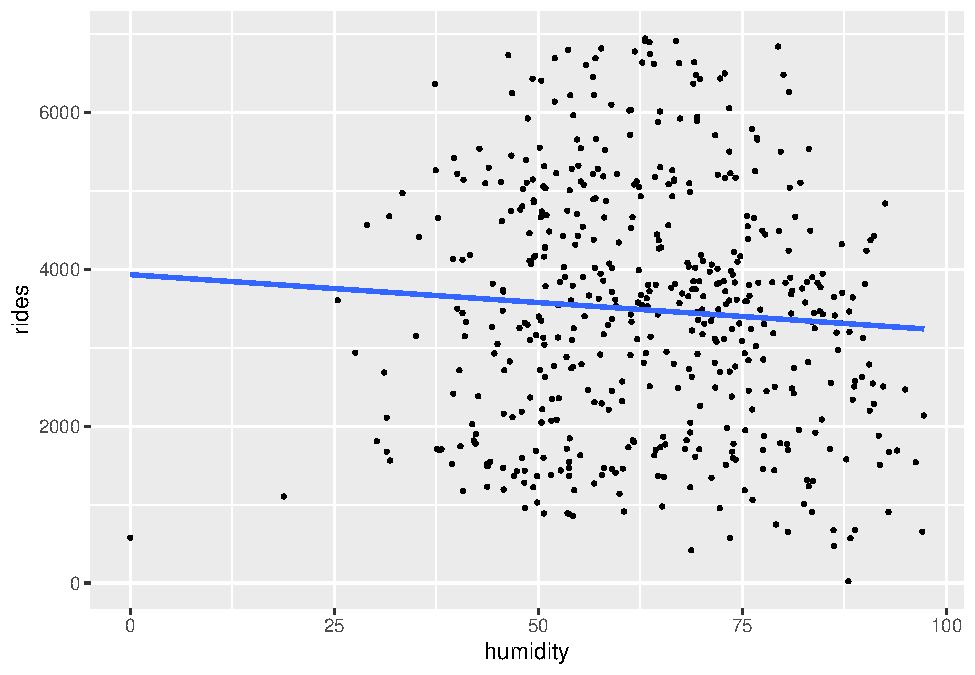
\includegraphics{HW-8_files/figure-latex/unnamed-chunk-8-1.pdf}

We can see that b gives a much better estimate than a.

\hypertarget{exercise-6.6}{%
\subsection{Exercise 6.6}\label{exercise-6.6}}

We're given a Gamma-Poison model for
Y\textbar lambda\textasciitilde Pois(lambda) and
lambda\textasciitilde Gamma(20,5). N = 3 and (Y1, Y2, Y3) = (0, 1, 0).

\begin{enumerate}
\def\labelenumi{\alph{enumi})}
\tightlist
\item
  Use grid approximation with values E\{0, 1, 2,\ldots8\} to approximate
  posterior model lambda.
\end{enumerate}

\begin{Shaded}
\begin{Highlighting}[]
\CommentTok{\# Step 1: Define a grid of 10 lambda values}
\NormalTok{grid\_data   }\OtherTok{\textless{}{-}} \FunctionTok{data.frame}\NormalTok{(}\AttributeTok{lambda\_grid =} \FunctionTok{seq}\NormalTok{(}\AttributeTok{from =} \DecValTok{0}\NormalTok{, }\AttributeTok{to =} \DecValTok{8}\NormalTok{, }\AttributeTok{length =} \DecValTok{8}\NormalTok{)) }

\CommentTok{\# Step 2: Evaluate the prior \& likelihood at each lambda}
\NormalTok{grid\_data }\OtherTok{\textless{}{-}}\NormalTok{ grid\_data }\SpecialCharTok{|}\ErrorTok{\textgreater{}} 
  \FunctionTok{mutate}\NormalTok{(}\AttributeTok{prior =} \FunctionTok{dgamma}\NormalTok{(lambda\_grid, }\DecValTok{20}\NormalTok{, }\DecValTok{5}\NormalTok{), }\CommentTok{\#given prior}
         \AttributeTok{likelihood =} \FunctionTok{dpois}\NormalTok{(}\DecValTok{0}\NormalTok{, lambda\_grid) }\SpecialCharTok{*} \FunctionTok{dpois}\NormalTok{(}\DecValTok{1}\NormalTok{, lambda\_grid) }\SpecialCharTok{*} \FunctionTok{dpois}\NormalTok{(}\DecValTok{0}\NormalTok{, lambda\_grid))}

\CommentTok{\# Step 3: Approximate the posterior}
\NormalTok{grid\_data }\OtherTok{\textless{}{-}}\NormalTok{ grid\_data }\SpecialCharTok{|}\ErrorTok{\textgreater{}} 
  \FunctionTok{mutate}\NormalTok{(}\AttributeTok{unnormalized =}\NormalTok{ likelihood }\SpecialCharTok{*}\NormalTok{ prior,}
         \AttributeTok{posterior =}\NormalTok{ unnormalized }\SpecialCharTok{/} \FunctionTok{sum}\NormalTok{(unnormalized))}

\CommentTok{\# Set the seed}
\FunctionTok{set.seed}\NormalTok{(}\DecValTok{1500}\NormalTok{)}

\CommentTok{\# Step 4: sample from the discretized posterior}
\NormalTok{post\_sample }\OtherTok{\textless{}{-}} \FunctionTok{sample\_n}\NormalTok{(grid\_data, }\AttributeTok{size =} \DecValTok{10000}\NormalTok{, }
                        \AttributeTok{weight =}\NormalTok{ posterior, }\AttributeTok{replace =} \ConstantTok{TRUE}\NormalTok{)}

\CommentTok{\#plotting histogram of the above }

\FunctionTok{ggplot}\NormalTok{(post\_sample, }\FunctionTok{aes}\NormalTok{(}\AttributeTok{x =}\NormalTok{ lambda\_grid)) }\SpecialCharTok{+} 
  \FunctionTok{geom\_histogram}\NormalTok{(}\FunctionTok{aes}\NormalTok{(}\AttributeTok{y =}\NormalTok{ ..density..), }\AttributeTok{color =} \StringTok{"white"}\NormalTok{) }\SpecialCharTok{+} 
  \FunctionTok{stat\_function}\NormalTok{(}\AttributeTok{fun =}\NormalTok{ dgamma, }\AttributeTok{args =} \FunctionTok{list}\NormalTok{(}\DecValTok{20}\NormalTok{, }\DecValTok{5}\NormalTok{)) }\SpecialCharTok{+} 
  \FunctionTok{lims}\NormalTok{(}\AttributeTok{x =} \FunctionTok{c}\NormalTok{(}\DecValTok{0}\NormalTok{, }\DecValTok{8}\NormalTok{))}
\end{Highlighting}
\end{Shaded}

\begin{verbatim}
## `stat_bin()` using `bins = 30`. Pick better value with `binwidth`.
\end{verbatim}

\begin{verbatim}
## Warning: Removed 2 rows containing missing values (geom_bar).
\end{verbatim}

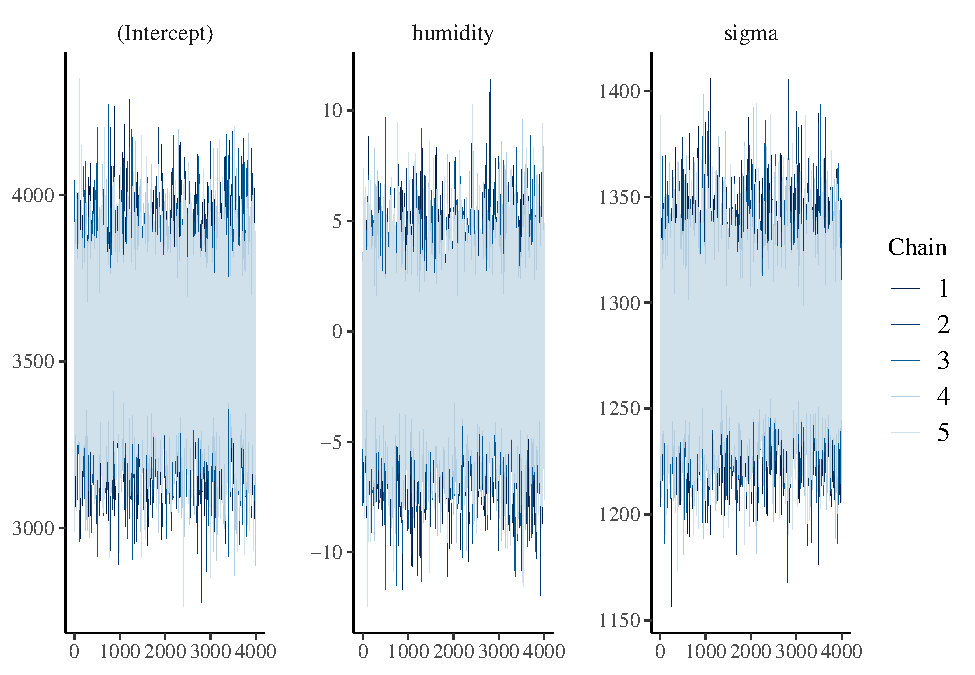
\includegraphics{HW-8_files/figure-latex/unnamed-chunk-9-1.pdf}

\begin{enumerate}
\def\labelenumi{\alph{enumi})}
\setcounter{enumi}{1}
\tightlist
\item
  Repeat the above using a grid of 201 with equally spaced values
  between 0 \& 8.
\end{enumerate}

\begin{Shaded}
\begin{Highlighting}[]
\CommentTok{\# Step 1: Define a grid of 10 lambda values}
\NormalTok{grid\_data   }\OtherTok{\textless{}{-}} \FunctionTok{data.frame}\NormalTok{(}\AttributeTok{lambda\_grid =} \FunctionTok{seq}\NormalTok{(}\AttributeTok{from =} \DecValTok{0}\NormalTok{, }\AttributeTok{to =} \DecValTok{8}\NormalTok{, }\AttributeTok{length =} \DecValTok{201}\NormalTok{)) }\CommentTok{\# went up to 10 values to see what happens after 8}

\CommentTok{\# Step 2: Evaluate the prior \& likelihood at each lambda}
\NormalTok{grid\_data }\OtherTok{\textless{}{-}}\NormalTok{ grid\_data }\SpecialCharTok{|}\ErrorTok{\textgreater{}} 
  \FunctionTok{mutate}\NormalTok{(}\AttributeTok{prior =} \FunctionTok{dgamma}\NormalTok{(lambda\_grid, }\DecValTok{20}\NormalTok{, }\DecValTok{5}\NormalTok{), }\CommentTok{\#given prior}
         \AttributeTok{likelihood =} \FunctionTok{dpois}\NormalTok{(}\DecValTok{0}\NormalTok{, lambda\_grid) }\SpecialCharTok{*} \FunctionTok{dpois}\NormalTok{(}\DecValTok{1}\NormalTok{, lambda\_grid) }\SpecialCharTok{*} \FunctionTok{dpois}\NormalTok{(}\DecValTok{0}\NormalTok{, lambda\_grid))}

\CommentTok{\# Step 3: Approximate the posterior}
\NormalTok{grid\_data }\OtherTok{\textless{}{-}}\NormalTok{ grid\_data }\SpecialCharTok{|}\ErrorTok{\textgreater{}} 
  \FunctionTok{mutate}\NormalTok{(}\AttributeTok{unnormalized =}\NormalTok{ likelihood }\SpecialCharTok{*}\NormalTok{ prior,}
         \AttributeTok{posterior =}\NormalTok{ unnormalized }\SpecialCharTok{/} \FunctionTok{sum}\NormalTok{(unnormalized))}

\CommentTok{\# Set the seed}
\FunctionTok{set.seed}\NormalTok{(}\DecValTok{1500}\NormalTok{)}

\CommentTok{\# Step 4: sample from the discretized posterior}
\NormalTok{post\_sample }\OtherTok{\textless{}{-}} \FunctionTok{sample\_n}\NormalTok{(grid\_data, }\AttributeTok{size =} \DecValTok{10000}\NormalTok{, }
                        \AttributeTok{weight =}\NormalTok{ posterior, }\AttributeTok{replace =} \ConstantTok{TRUE}\NormalTok{)}

\CommentTok{\#plotting histogram of the above }

\FunctionTok{ggplot}\NormalTok{(post\_sample, }\FunctionTok{aes}\NormalTok{(}\AttributeTok{x =}\NormalTok{ lambda\_grid)) }\SpecialCharTok{+} 
  \FunctionTok{geom\_histogram}\NormalTok{(}\FunctionTok{aes}\NormalTok{(}\AttributeTok{y =}\NormalTok{ ..density..), }\AttributeTok{color =} \StringTok{"white"}\NormalTok{) }\SpecialCharTok{+} 
  \FunctionTok{stat\_function}\NormalTok{(}\AttributeTok{fun =}\NormalTok{ dgamma, }\AttributeTok{args =} \FunctionTok{list}\NormalTok{(}\DecValTok{20}\NormalTok{, }\DecValTok{5}\NormalTok{)) }\SpecialCharTok{+} 
  \FunctionTok{lims}\NormalTok{(}\AttributeTok{x =} \FunctionTok{c}\NormalTok{(}\DecValTok{0}\NormalTok{, }\DecValTok{8}\NormalTok{))}
\end{Highlighting}
\end{Shaded}

\begin{verbatim}
## `stat_bin()` using `bins = 30`. Pick better value with `binwidth`.
\end{verbatim}

\begin{verbatim}
## Warning: Removed 2 rows containing missing values (geom_bar).
\end{verbatim}

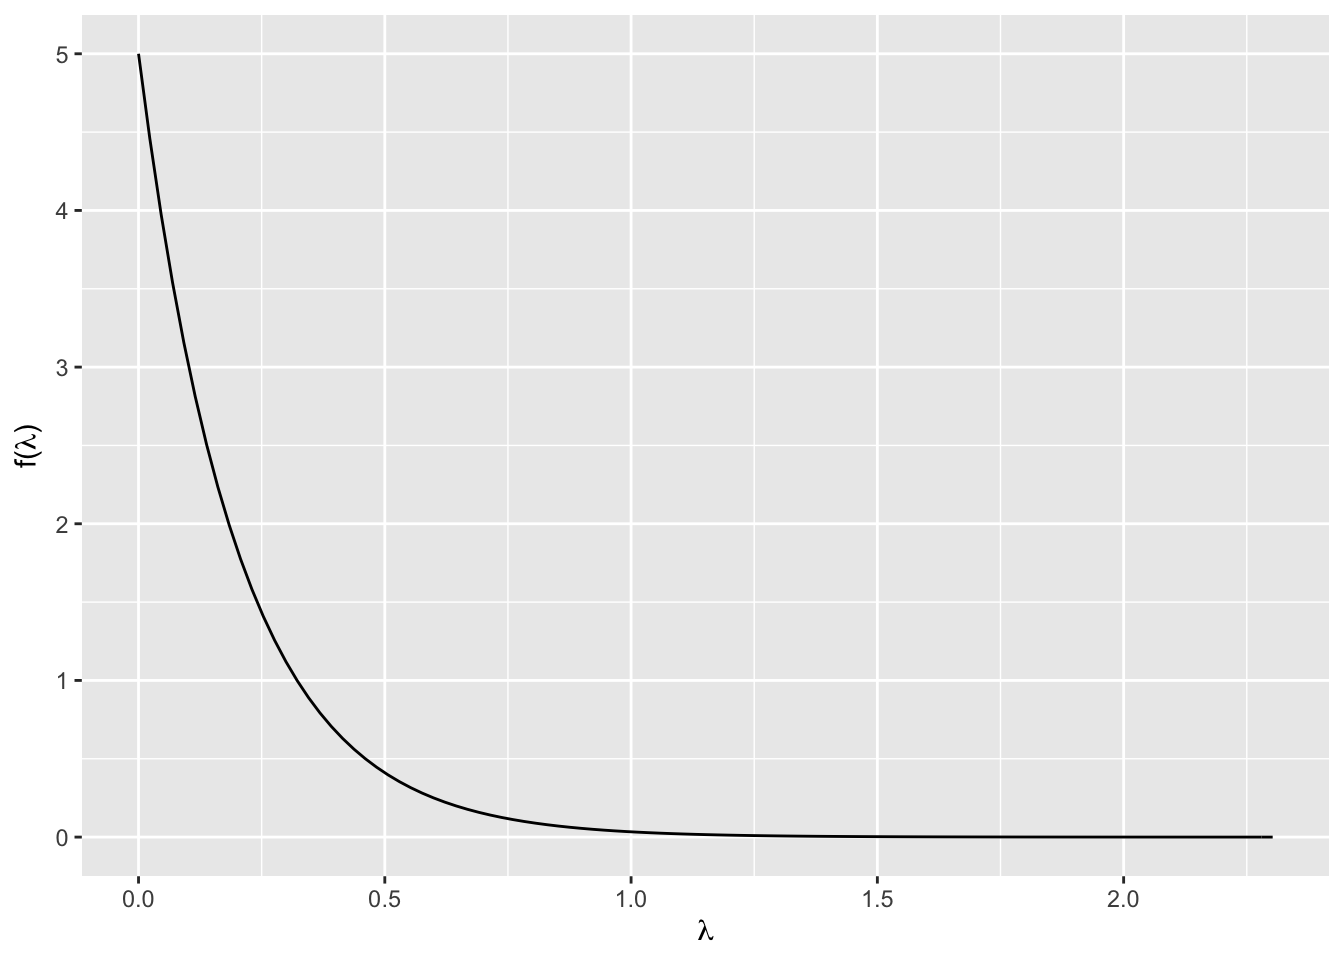
\includegraphics{HW-8_files/figure-latex/unnamed-chunk-10-1.pdf} \#\#
Exercise 6.7

We're given a normal-normal model for mu with
Y\textbar mu\textasciitilde N(mu, 1.3\^{}2) and
mu\textasciitilde N(10,1.2\^{}2). Observed data is (Y1, Y2, Y3, Y4) =
(7.1, 8.9, 8.4, 8.6)

\begin{Shaded}
\begin{Highlighting}[]
\CommentTok{\# Step 1: Define a grid of 50 mu values}
\NormalTok{grid\_data  }\OtherTok{\textless{}{-}} \FunctionTok{data.frame}\NormalTok{(}\AttributeTok{mu\_grid =} \FunctionTok{seq}\NormalTok{(}\AttributeTok{from =} \DecValTok{7}\NormalTok{, }\AttributeTok{to =} \DecValTok{10}\NormalTok{, }\AttributeTok{length =} \DecValTok{50}\NormalTok{)) }\CommentTok{\#narrowed the sequence range }
\CommentTok{\#changed to 50 values to demonstrate that I know as grid spacing decreases, quality of approximation decreases }

\CommentTok{\# Step 2: Evaluate the prior \& likelihood at each mu}
\NormalTok{grid\_data }\OtherTok{\textless{}{-}}\NormalTok{ grid\_data }\SpecialCharTok{|}\ErrorTok{\textgreater{}} 
  \FunctionTok{mutate}\NormalTok{(}\AttributeTok{prior =} \FunctionTok{dnorm}\NormalTok{(mu\_grid, }\AttributeTok{mean =} \DecValTok{10}\NormalTok{, }\AttributeTok{sd =} \FloatTok{1.2}\NormalTok{), }
         \AttributeTok{likelihood =} \FunctionTok{dnorm}\NormalTok{(}\FloatTok{7.1}\NormalTok{, }\AttributeTok{mean =}\NormalTok{ mu\_grid, }\AttributeTok{sd =} \FloatTok{1.3}\NormalTok{)}\SpecialCharTok{*}
           \FunctionTok{dnorm}\NormalTok{(}\FloatTok{8.9}\NormalTok{, }\AttributeTok{mean =}\NormalTok{ mu\_grid, }\AttributeTok{sd =} \FloatTok{1.3}\NormalTok{)}\SpecialCharTok{*} 
           \FunctionTok{dnorm}\NormalTok{(}\FloatTok{8.4}\NormalTok{, }\AttributeTok{mean =}\NormalTok{ mu\_grid, }\AttributeTok{sd =} \FloatTok{1.3}\NormalTok{)}\SpecialCharTok{*} 
           \FunctionTok{dnorm}\NormalTok{(}\FloatTok{8.6}\NormalTok{, }\AttributeTok{mean =}\NormalTok{ mu\_grid, }\AttributeTok{sd =} \FloatTok{1.3}\NormalTok{))}


\CommentTok{\# Step 3: Approximate the posterior}
\NormalTok{grid\_data }\OtherTok{\textless{}{-}}\NormalTok{ grid\_data }\SpecialCharTok{|}\ErrorTok{\textgreater{}}  
  \FunctionTok{mutate}\NormalTok{(}\AttributeTok{unnormalized =}\NormalTok{ likelihood }\SpecialCharTok{*}\NormalTok{ prior,}
         \AttributeTok{posterior =}\NormalTok{ unnormalized }\SpecialCharTok{/} \FunctionTok{sum}\NormalTok{(unnormalized))}

\FunctionTok{ggplot}\NormalTok{(grid\_data, }\FunctionTok{aes}\NormalTok{(}\AttributeTok{x =}\NormalTok{ mu\_grid, }\AttributeTok{y =}\NormalTok{ posterior)) }\SpecialCharTok{+} 
  \FunctionTok{geom\_point}\NormalTok{() }\SpecialCharTok{+} 
  \FunctionTok{geom\_segment}\NormalTok{(}\FunctionTok{aes}\NormalTok{(}\AttributeTok{x =}\NormalTok{ mu\_grid, }\AttributeTok{xend =}\NormalTok{ mu\_grid, }\AttributeTok{y =} \DecValTok{0}\NormalTok{, }\AttributeTok{yend =}\NormalTok{ posterior))}
\end{Highlighting}
\end{Shaded}

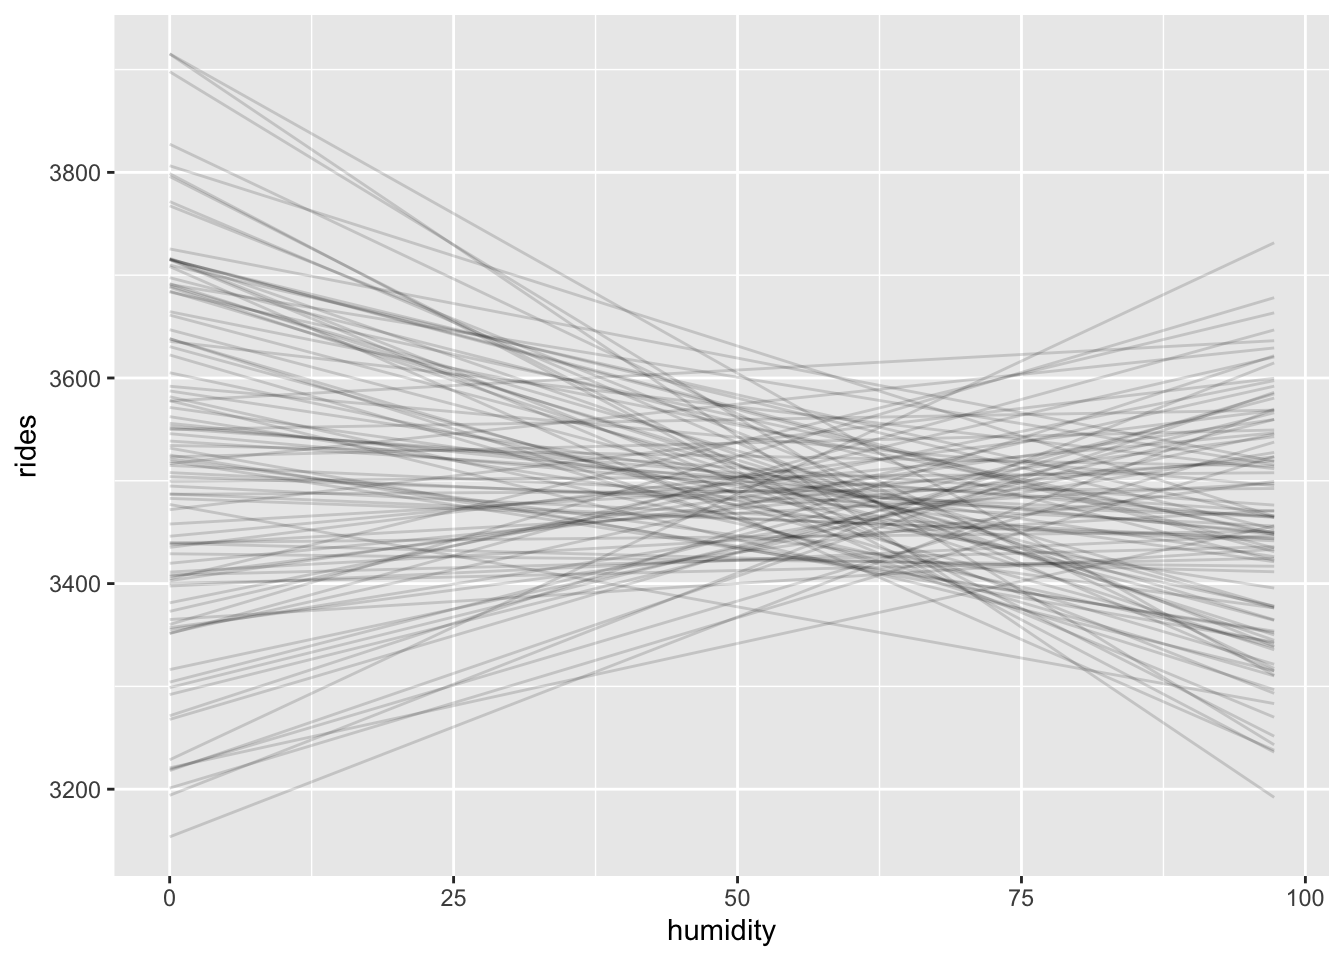
\includegraphics{HW-8_files/figure-latex/unnamed-chunk-11-1.pdf}

\begin{enumerate}
\def\labelenumi{\alph{enumi})}
\setcounter{enumi}{1}
\tightlist
\item
  Repeat the above using a grid of 201 equally spaced values b/w 5 and
  15.
\end{enumerate}

\begin{Shaded}
\begin{Highlighting}[]
\CommentTok{\# Step 1: Define a grid of 201 mu values}
\NormalTok{grid\_data  }\OtherTok{\textless{}{-}} \FunctionTok{data.frame}\NormalTok{(}\AttributeTok{mu\_grid =} \FunctionTok{seq}\NormalTok{(}\AttributeTok{from =} \DecValTok{5}\NormalTok{, }\AttributeTok{to =} \DecValTok{15}\NormalTok{, }\AttributeTok{length =} \DecValTok{201}\NormalTok{)) }

\CommentTok{\# Step 2: Evaluate the prior \& likelihood at each mu}
\NormalTok{grid\_data }\OtherTok{\textless{}{-}}\NormalTok{ grid\_data }\SpecialCharTok{|}\ErrorTok{\textgreater{}} 
  \FunctionTok{mutate}\NormalTok{(}\AttributeTok{prior =} \FunctionTok{dnorm}\NormalTok{(mu\_grid, }\AttributeTok{mean =} \DecValTok{10}\NormalTok{, }\AttributeTok{sd =} \FloatTok{1.2}\NormalTok{), }
         \AttributeTok{likelihood =} \FunctionTok{dnorm}\NormalTok{(}\FloatTok{7.1}\NormalTok{, }\AttributeTok{mean =}\NormalTok{ mu\_grid, }\AttributeTok{sd =} \FloatTok{1.3}\NormalTok{)}\SpecialCharTok{*}
           \FunctionTok{dnorm}\NormalTok{(}\FloatTok{8.9}\NormalTok{, }\AttributeTok{mean =}\NormalTok{ mu\_grid, }\AttributeTok{sd =} \FloatTok{1.3}\NormalTok{)}\SpecialCharTok{*} 
           \FunctionTok{dnorm}\NormalTok{(}\FloatTok{8.4}\NormalTok{, }\AttributeTok{mean =}\NormalTok{ mu\_grid, }\AttributeTok{sd =} \FloatTok{1.3}\NormalTok{)}\SpecialCharTok{*} 
           \FunctionTok{dnorm}\NormalTok{(}\FloatTok{8.6}\NormalTok{, }\AttributeTok{mean =}\NormalTok{ mu\_grid, }\AttributeTok{sd =} \FloatTok{1.3}\NormalTok{))}


\CommentTok{\# Step 3: Approximate the posterior}
\NormalTok{grid\_data }\OtherTok{\textless{}{-}}\NormalTok{ grid\_data }\SpecialCharTok{|}\ErrorTok{\textgreater{}}  
  \FunctionTok{mutate}\NormalTok{(}\AttributeTok{unnormalized =}\NormalTok{ likelihood }\SpecialCharTok{*}\NormalTok{ prior,}
         \AttributeTok{posterior =}\NormalTok{ unnormalized }\SpecialCharTok{/} \FunctionTok{sum}\NormalTok{(unnormalized))}

\FunctionTok{ggplot}\NormalTok{(grid\_data, }\FunctionTok{aes}\NormalTok{(}\AttributeTok{x =}\NormalTok{ mu\_grid, }\AttributeTok{y =}\NormalTok{ posterior)) }\SpecialCharTok{+} 
  \FunctionTok{geom\_point}\NormalTok{() }\SpecialCharTok{+} 
  \FunctionTok{geom\_segment}\NormalTok{(}\FunctionTok{aes}\NormalTok{(}\AttributeTok{x =}\NormalTok{ mu\_grid, }\AttributeTok{xend =}\NormalTok{ mu\_grid, }\AttributeTok{y =} \DecValTok{0}\NormalTok{, }\AttributeTok{yend =}\NormalTok{ posterior))}
\end{Highlighting}
\end{Shaded}

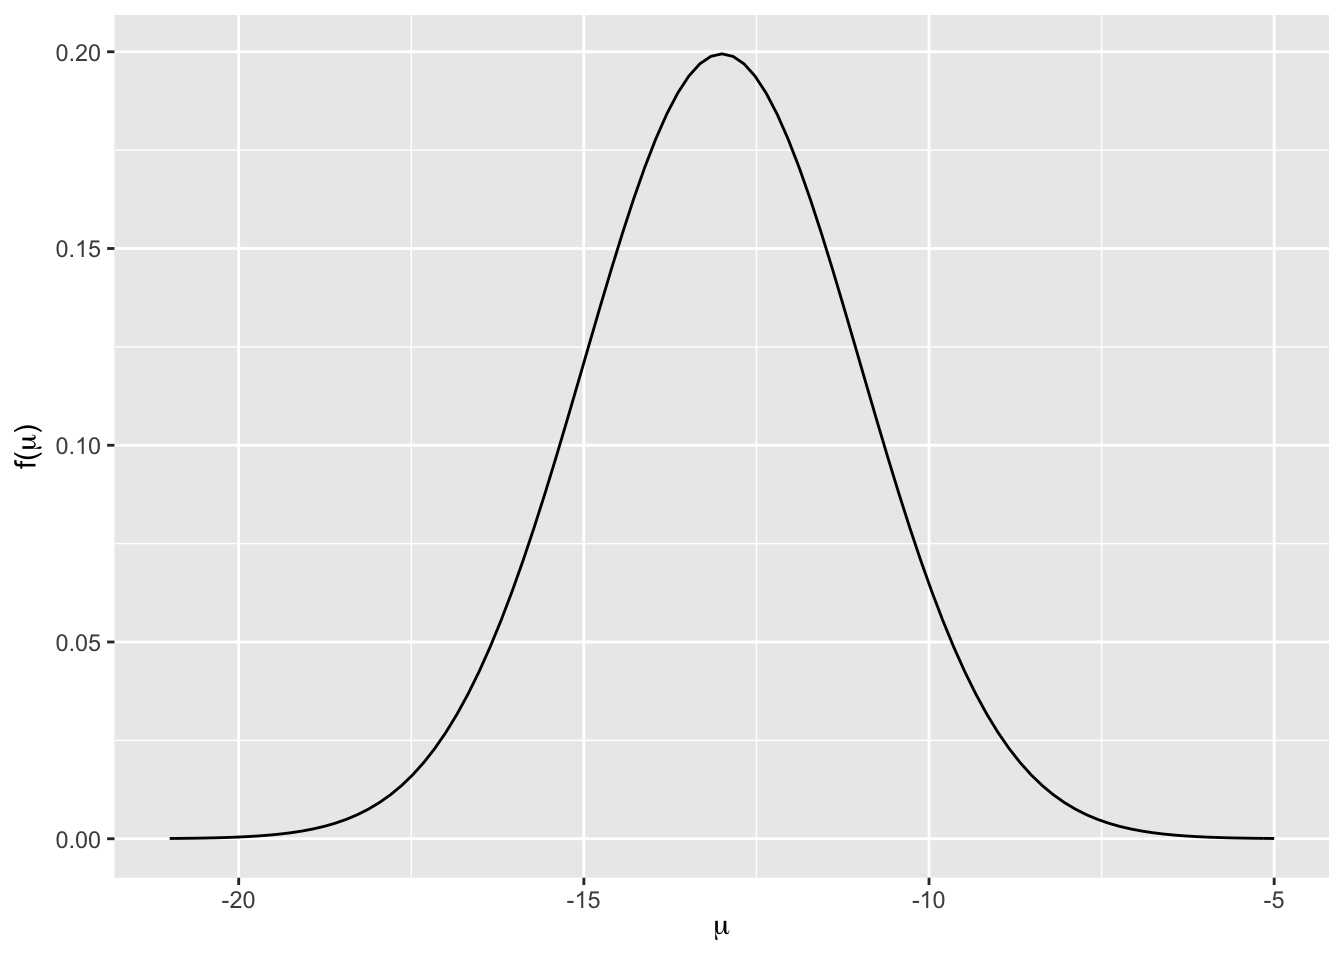
\includegraphics{HW-8_files/figure-latex/unnamed-chunk-12-1.pdf}

\hypertarget{exercise-6.8}{%
\subsection{Exercise 6.8}\label{exercise-6.8}}

\begin{enumerate}
\def\labelenumi{\alph{enumi})}
\item
  A high dimensional Bayesian model could be useful for analyzing how
  well a medication works over time across different patients. The
  dimensions are time/age of patient and symptoms; there will be
  different symptoms across patients and across time.
\item
  The issue with dimensionality is that even for 2 dimensions, there
  could be an enormous scale of approximations to make because
  approximations would need to be calculated for both the x and y axis.
  If we had 100 values for the x-dimension and 100 for the y-dimension
  that would be 10,000 approximations. This may be timely and is
  inefficient to run as dimensions and number of values increase.
\end{enumerate}

\hypertarget{exercise-6.9}{%
\subsection{Exercise 6.9}\label{exercise-6.9}}

\begin{enumerate}
\def\labelenumi{\alph{enumi})}
\item
  The drawback for both grid approximations and MCMC are that they are
  discretized approximations. We should remember this when using these
  methods for continuous data.
\item
  The advantage of both MCMC and grid approximation are that they allow
  for approximations for posteriors that are difficult to solve by-hand.
\item
  An advantage that grid has over MCMC is that the code seems generally
  easier to write and can be done in R (without using Rstan and
  associated C++ issues).
\item
  An advantage of MCMC over grid approximation is the ability to
  estimate posteriors for multiple dimensions.
\end{enumerate}

\hypertarget{exercise-6.10}{%
\subsection{Exercise 6.10}\label{exercise-6.10}}

For something to be a Markov chain, event i is dependent only on i-1.
There is memorylessness and otherwise independence for the event for
i-2, i-3, and so on.

\begin{enumerate}
\def\labelenumi{\alph{enumi})}
\item
  This scenario is not an Markov chain if I assume that the first
  several nights in a row involved me going to a Thai restaurant. The
  prior frequency of Thai restaurants (on days i-2, i-3, etc.) may
  influence my choice on day i.
\item
  This is also not a Markov chain because there is complete independence
  from day to day for winning the lottery. Markov chains need i to be
  dependent on i-1.
\item
  This is not a Markov chain for similar reasons to a. There is memory
  about i-2, i-3, etc., i.e.~an experienced chess player does remember
  the prior moves of other players. If the players are not good and can
  only remember the last game they played, then this could be a Markov
  chain.
\end{enumerate}

\hypertarget{exercise-6.11}{%
\subsection{Exercise 6.11}\label{exercise-6.11}}

Use information to write RStan syntax.

\begin{enumerate}
\def\labelenumi{\alph{enumi})}
\tightlist
\item
\end{enumerate}

\begin{Shaded}
\begin{Highlighting}[]
\CommentTok{\# STEP 1: Define beta{-}binomial model assuming 12 trials }
\NormalTok{bb\_model }\OtherTok{\textless{}{-}} \StringTok{"}
\StringTok{  data \{}
\StringTok{    int\textless{}lower = 0, upper = 12\textgreater{} Y;}
\StringTok{  \}}
\StringTok{  parameters \{}
\StringTok{    real\textless{}lower = 0, upper = 1\textgreater{} pi;}
\StringTok{  \}}
\StringTok{  model \{}
\StringTok{    Y \textasciitilde{} binomial(20, pi);}
\StringTok{    pi \textasciitilde{} beta(1, 1);}
\StringTok{  \}}
\StringTok{  "}
\end{Highlighting}
\end{Shaded}

\begin{enumerate}
\def\labelenumi{\alph{enumi})}
\setcounter{enumi}{1}
\tightlist
\item
\end{enumerate}

\begin{Shaded}
\begin{Highlighting}[]
\CommentTok{\# STEP 1: Define Gamma{-}Poisson model in stan syntax }
\NormalTok{gp\_model }\OtherTok{\textless{}{-}} \StringTok{"}
\StringTok{  data \{}
\StringTok{    int\textless{}lower = 0\textgreater{} Y[3];}
\StringTok{  \}}
\StringTok{  parameters \{}
\StringTok{    real\textless{}lower = 0\textgreater{} lambda;}
\StringTok{  \}}
\StringTok{  model \{}
\StringTok{    Y \textasciitilde{} poisson(lambda);}
\StringTok{    lambda \textasciitilde{} gamma(4, 2);}
\StringTok{  \}}
\StringTok{"}
\end{Highlighting}
\end{Shaded}

\begin{enumerate}
\def\labelenumi{\alph{enumi})}
\setcounter{enumi}{2}
\tightlist
\item
\end{enumerate}

\begin{Shaded}
\begin{Highlighting}[]
\NormalTok{normal\_model }\OtherTok{\textless{}{-}} \StringTok{"}
\StringTok{data \{}
\StringTok{    vector[4] Y; }
\StringTok{\} }
\StringTok{parameters \{}
\StringTok{    real mu;}
\StringTok{\} }
\StringTok{model \{}
\StringTok{   Y \textasciitilde{} normal(mu, 1\^{}2);}
\StringTok{   mu \textasciitilde{} normal(0, 10\^{}2);}
\StringTok{\}}
\StringTok{"}
\end{Highlighting}
\end{Shaded}

\hypertarget{exercise-6.12}{%
\subsection{Exercise 6.12}\label{exercise-6.12}}

Write the Rstan syntax for simulating the posterior.

\begin{Shaded}
\begin{Highlighting}[]
\CommentTok{\#a}
\NormalTok{bb\_sim }\OtherTok{\textless{}{-}} \FunctionTok{stan}\NormalTok{(}\AttributeTok{model\_code =}\NormalTok{ bb\_model, }\AttributeTok{data =} \FunctionTok{list}\NormalTok{(}\AttributeTok{Y =} \DecValTok{12}\NormalTok{), }
               \AttributeTok{chains =} \DecValTok{4}\NormalTok{, }\AttributeTok{iter =} \DecValTok{1000}\SpecialCharTok{*}\DecValTok{2}\NormalTok{, }\AttributeTok{seed =} \DecValTok{100}\NormalTok{) }\CommentTok{\#chose 1000 to reduce processing time}
\end{Highlighting}
\end{Shaded}

\begin{verbatim}
## Trying to compile a simple C file
\end{verbatim}

\begin{verbatim}
## Running /Library/Frameworks/R.framework/Resources/bin/R CMD SHLIB foo.c
## clang -arch arm64 -I"/Library/Frameworks/R.framework/Resources/include" -DNDEBUG   -I"/Library/Frameworks/R.framework/Versions/4.1-arm64/Resources/library/Rcpp/include/"  -I"/Library/Frameworks/R.framework/Versions/4.1-arm64/Resources/library/RcppEigen/include/"  -I"/Library/Frameworks/R.framework/Versions/4.1-arm64/Resources/library/RcppEigen/include/unsupported"  -I"/Library/Frameworks/R.framework/Versions/4.1-arm64/Resources/library/BH/include" -I"/Library/Frameworks/R.framework/Versions/4.1-arm64/Resources/library/StanHeaders/include/src/"  -I"/Library/Frameworks/R.framework/Versions/4.1-arm64/Resources/library/StanHeaders/include/"  -I"/Library/Frameworks/R.framework/Versions/4.1-arm64/Resources/library/RcppParallel/include/"  -I"/Library/Frameworks/R.framework/Versions/4.1-arm64/Resources/library/rstan/include" -DEIGEN_NO_DEBUG  -DBOOST_DISABLE_ASSERTS  -DBOOST_PENDING_INTEGER_LOG2_HPP  -DSTAN_THREADS  -DBOOST_NO_AUTO_PTR  -include '/Library/Frameworks/R.framework/Versions/4.1-arm64/Resources/library/StanHeaders/include/stan/math/prim/mat/fun/Eigen.hpp'  -D_REENTRANT -DRCPP_PARALLEL_USE_TBB=1   -I/opt/R/arm64/include   -fPIC  -falign-functions=64 -Wall -g -O2  -c foo.c -o foo.o
## In file included from <built-in>:1:
## In file included from /Library/Frameworks/R.framework/Versions/4.1-arm64/Resources/library/StanHeaders/include/stan/math/prim/mat/fun/Eigen.hpp:13:
## In file included from /Library/Frameworks/R.framework/Versions/4.1-arm64/Resources/library/RcppEigen/include/Eigen/Dense:1:
## In file included from /Library/Frameworks/R.framework/Versions/4.1-arm64/Resources/library/RcppEigen/include/Eigen/Core:88:
## /Library/Frameworks/R.framework/Versions/4.1-arm64/Resources/library/RcppEigen/include/Eigen/src/Core/util/Macros.h:628:1: error: unknown type name 'namespace'
## namespace Eigen {
## ^
## /Library/Frameworks/R.framework/Versions/4.1-arm64/Resources/library/RcppEigen/include/Eigen/src/Core/util/Macros.h:628:16: error: expected ';' after top level declarator
## namespace Eigen {
##                ^
##                ;
## In file included from <built-in>:1:
## In file included from /Library/Frameworks/R.framework/Versions/4.1-arm64/Resources/library/StanHeaders/include/stan/math/prim/mat/fun/Eigen.hpp:13:
## In file included from /Library/Frameworks/R.framework/Versions/4.1-arm64/Resources/library/RcppEigen/include/Eigen/Dense:1:
## /Library/Frameworks/R.framework/Versions/4.1-arm64/Resources/library/RcppEigen/include/Eigen/Core:96:10: fatal error: 'complex' file not found
## #include <complex>
##          ^~~~~~~~~
## 3 errors generated.
## make: *** [foo.o] Error 1
## 
## SAMPLING FOR MODEL 'f00f04dd6e1d8d07874d547d5cc1ea7b' NOW (CHAIN 1).
## Chain 1: 
## Chain 1: Gradient evaluation took 7e-06 seconds
## Chain 1: 1000 transitions using 10 leapfrog steps per transition would take 0.07 seconds.
## Chain 1: Adjust your expectations accordingly!
## Chain 1: 
## Chain 1: 
## Chain 1: Iteration:    1 / 2000 [  0%]  (Warmup)
## Chain 1: Iteration:  200 / 2000 [ 10%]  (Warmup)
## Chain 1: Iteration:  400 / 2000 [ 20%]  (Warmup)
## Chain 1: Iteration:  600 / 2000 [ 30%]  (Warmup)
## Chain 1: Iteration:  800 / 2000 [ 40%]  (Warmup)
## Chain 1: Iteration: 1000 / 2000 [ 50%]  (Warmup)
## Chain 1: Iteration: 1001 / 2000 [ 50%]  (Sampling)
## Chain 1: Iteration: 1200 / 2000 [ 60%]  (Sampling)
## Chain 1: Iteration: 1400 / 2000 [ 70%]  (Sampling)
## Chain 1: Iteration: 1600 / 2000 [ 80%]  (Sampling)
## Chain 1: Iteration: 1800 / 2000 [ 90%]  (Sampling)
## Chain 1: Iteration: 2000 / 2000 [100%]  (Sampling)
## Chain 1: 
## Chain 1:  Elapsed Time: 0.004937 seconds (Warm-up)
## Chain 1:                0.004574 seconds (Sampling)
## Chain 1:                0.009511 seconds (Total)
## Chain 1: 
## 
## SAMPLING FOR MODEL 'f00f04dd6e1d8d07874d547d5cc1ea7b' NOW (CHAIN 2).
## Chain 2: 
## Chain 2: Gradient evaluation took 4e-06 seconds
## Chain 2: 1000 transitions using 10 leapfrog steps per transition would take 0.04 seconds.
## Chain 2: Adjust your expectations accordingly!
## Chain 2: 
## Chain 2: 
## Chain 2: Iteration:    1 / 2000 [  0%]  (Warmup)
## Chain 2: Iteration:  200 / 2000 [ 10%]  (Warmup)
## Chain 2: Iteration:  400 / 2000 [ 20%]  (Warmup)
## Chain 2: Iteration:  600 / 2000 [ 30%]  (Warmup)
## Chain 2: Iteration:  800 / 2000 [ 40%]  (Warmup)
## Chain 2: Iteration: 1000 / 2000 [ 50%]  (Warmup)
## Chain 2: Iteration: 1001 / 2000 [ 50%]  (Sampling)
## Chain 2: Iteration: 1200 / 2000 [ 60%]  (Sampling)
## Chain 2: Iteration: 1400 / 2000 [ 70%]  (Sampling)
## Chain 2: Iteration: 1600 / 2000 [ 80%]  (Sampling)
## Chain 2: Iteration: 1800 / 2000 [ 90%]  (Sampling)
## Chain 2: Iteration: 2000 / 2000 [100%]  (Sampling)
## Chain 2: 
## Chain 2:  Elapsed Time: 0.004729 seconds (Warm-up)
## Chain 2:                0.004624 seconds (Sampling)
## Chain 2:                0.009353 seconds (Total)
## Chain 2: 
## 
## SAMPLING FOR MODEL 'f00f04dd6e1d8d07874d547d5cc1ea7b' NOW (CHAIN 3).
## Chain 3: 
## Chain 3: Gradient evaluation took 1e-06 seconds
## Chain 3: 1000 transitions using 10 leapfrog steps per transition would take 0.01 seconds.
## Chain 3: Adjust your expectations accordingly!
## Chain 3: 
## Chain 3: 
## Chain 3: Iteration:    1 / 2000 [  0%]  (Warmup)
## Chain 3: Iteration:  200 / 2000 [ 10%]  (Warmup)
## Chain 3: Iteration:  400 / 2000 [ 20%]  (Warmup)
## Chain 3: Iteration:  600 / 2000 [ 30%]  (Warmup)
## Chain 3: Iteration:  800 / 2000 [ 40%]  (Warmup)
## Chain 3: Iteration: 1000 / 2000 [ 50%]  (Warmup)
## Chain 3: Iteration: 1001 / 2000 [ 50%]  (Sampling)
## Chain 3: Iteration: 1200 / 2000 [ 60%]  (Sampling)
## Chain 3: Iteration: 1400 / 2000 [ 70%]  (Sampling)
## Chain 3: Iteration: 1600 / 2000 [ 80%]  (Sampling)
## Chain 3: Iteration: 1800 / 2000 [ 90%]  (Sampling)
## Chain 3: Iteration: 2000 / 2000 [100%]  (Sampling)
## Chain 3: 
## Chain 3:  Elapsed Time: 0.004728 seconds (Warm-up)
## Chain 3:                0.004674 seconds (Sampling)
## Chain 3:                0.009402 seconds (Total)
## Chain 3: 
## 
## SAMPLING FOR MODEL 'f00f04dd6e1d8d07874d547d5cc1ea7b' NOW (CHAIN 4).
## Chain 4: 
## Chain 4: Gradient evaluation took 1e-06 seconds
## Chain 4: 1000 transitions using 10 leapfrog steps per transition would take 0.01 seconds.
## Chain 4: Adjust your expectations accordingly!
## Chain 4: 
## Chain 4: 
## Chain 4: Iteration:    1 / 2000 [  0%]  (Warmup)
## Chain 4: Iteration:  200 / 2000 [ 10%]  (Warmup)
## Chain 4: Iteration:  400 / 2000 [ 20%]  (Warmup)
## Chain 4: Iteration:  600 / 2000 [ 30%]  (Warmup)
## Chain 4: Iteration:  800 / 2000 [ 40%]  (Warmup)
## Chain 4: Iteration: 1000 / 2000 [ 50%]  (Warmup)
## Chain 4: Iteration: 1001 / 2000 [ 50%]  (Sampling)
## Chain 4: Iteration: 1200 / 2000 [ 60%]  (Sampling)
## Chain 4: Iteration: 1400 / 2000 [ 70%]  (Sampling)
## Chain 4: Iteration: 1600 / 2000 [ 80%]  (Sampling)
## Chain 4: Iteration: 1800 / 2000 [ 90%]  (Sampling)
## Chain 4: Iteration: 2000 / 2000 [100%]  (Sampling)
## Chain 4: 
## Chain 4:  Elapsed Time: 0.004747 seconds (Warm-up)
## Chain 4:                0.004258 seconds (Sampling)
## Chain 4:                0.009005 seconds (Total)
## Chain 4:
\end{verbatim}

\begin{Shaded}
\begin{Highlighting}[]
\CommentTok{\#b}
\NormalTok{gp\_sim }\OtherTok{\textless{}{-}} \FunctionTok{stan}\NormalTok{(}\AttributeTok{model\_code =}\NormalTok{ gp\_model, }\AttributeTok{data =} \FunctionTok{list}\NormalTok{(}\AttributeTok{Y =} \FunctionTok{c}\NormalTok{(}\DecValTok{3}\NormalTok{)), }
               \AttributeTok{chains =} \DecValTok{4}\NormalTok{, }\AttributeTok{iter =} \DecValTok{1000}\SpecialCharTok{*}\DecValTok{2}\NormalTok{, }\AttributeTok{seed =} \DecValTok{200}\NormalTok{)}
\end{Highlighting}
\end{Shaded}

\begin{verbatim}
## Trying to compile a simple C file
\end{verbatim}

\begin{verbatim}
## Running /Library/Frameworks/R.framework/Resources/bin/R CMD SHLIB foo.c
## clang -arch arm64 -I"/Library/Frameworks/R.framework/Resources/include" -DNDEBUG   -I"/Library/Frameworks/R.framework/Versions/4.1-arm64/Resources/library/Rcpp/include/"  -I"/Library/Frameworks/R.framework/Versions/4.1-arm64/Resources/library/RcppEigen/include/"  -I"/Library/Frameworks/R.framework/Versions/4.1-arm64/Resources/library/RcppEigen/include/unsupported"  -I"/Library/Frameworks/R.framework/Versions/4.1-arm64/Resources/library/BH/include" -I"/Library/Frameworks/R.framework/Versions/4.1-arm64/Resources/library/StanHeaders/include/src/"  -I"/Library/Frameworks/R.framework/Versions/4.1-arm64/Resources/library/StanHeaders/include/"  -I"/Library/Frameworks/R.framework/Versions/4.1-arm64/Resources/library/RcppParallel/include/"  -I"/Library/Frameworks/R.framework/Versions/4.1-arm64/Resources/library/rstan/include" -DEIGEN_NO_DEBUG  -DBOOST_DISABLE_ASSERTS  -DBOOST_PENDING_INTEGER_LOG2_HPP  -DSTAN_THREADS  -DBOOST_NO_AUTO_PTR  -include '/Library/Frameworks/R.framework/Versions/4.1-arm64/Resources/library/StanHeaders/include/stan/math/prim/mat/fun/Eigen.hpp'  -D_REENTRANT -DRCPP_PARALLEL_USE_TBB=1   -I/opt/R/arm64/include   -fPIC  -falign-functions=64 -Wall -g -O2  -c foo.c -o foo.o
## In file included from <built-in>:1:
## In file included from /Library/Frameworks/R.framework/Versions/4.1-arm64/Resources/library/StanHeaders/include/stan/math/prim/mat/fun/Eigen.hpp:13:
## In file included from /Library/Frameworks/R.framework/Versions/4.1-arm64/Resources/library/RcppEigen/include/Eigen/Dense:1:
## In file included from /Library/Frameworks/R.framework/Versions/4.1-arm64/Resources/library/RcppEigen/include/Eigen/Core:88:
## /Library/Frameworks/R.framework/Versions/4.1-arm64/Resources/library/RcppEigen/include/Eigen/src/Core/util/Macros.h:628:1: error: unknown type name 'namespace'
## namespace Eigen {
## ^
## /Library/Frameworks/R.framework/Versions/4.1-arm64/Resources/library/RcppEigen/include/Eigen/src/Core/util/Macros.h:628:16: error: expected ';' after top level declarator
## namespace Eigen {
##                ^
##                ;
## In file included from <built-in>:1:
## In file included from /Library/Frameworks/R.framework/Versions/4.1-arm64/Resources/library/StanHeaders/include/stan/math/prim/mat/fun/Eigen.hpp:13:
## In file included from /Library/Frameworks/R.framework/Versions/4.1-arm64/Resources/library/RcppEigen/include/Eigen/Dense:1:
## /Library/Frameworks/R.framework/Versions/4.1-arm64/Resources/library/RcppEigen/include/Eigen/Core:96:10: fatal error: 'complex' file not found
## #include <complex>
##          ^~~~~~~~~
## 3 errors generated.
## make: *** [foo.o] Error 1
## Error in mod$fit_ptr() : 
##   Exception: mismatch in number dimensions declared and found in context; processing stage=data initialization; variable name=Y; dims declared=(3); dims found=()  (in 'model290e689fb08e_ef4eccd314be26b89d367d636885a01c' at line 3)
\end{verbatim}

\begin{verbatim}
## failed to create the sampler; sampling not done
\end{verbatim}

\begin{Shaded}
\begin{Highlighting}[]
\CommentTok{\#c}
\NormalTok{d }\OtherTok{\textless{}{-}} \FunctionTok{list}\NormalTok{(}\AttributeTok{Y =} \FunctionTok{c}\NormalTok{(}\FloatTok{12.2}\NormalTok{))}
\NormalTok{nn\_sim }\OtherTok{\textless{}{-}} \FunctionTok{stan}\NormalTok{(}\AttributeTok{model\_code =}\NormalTok{ normal\_model, }\AttributeTok{data =}\NormalTok{ d, }
               \AttributeTok{chains =} \DecValTok{4}\NormalTok{, }\AttributeTok{iter =} \DecValTok{1000}\SpecialCharTok{*}\DecValTok{2}\NormalTok{, }\AttributeTok{seed =} \DecValTok{300}\NormalTok{)}
\end{Highlighting}
\end{Shaded}

\begin{verbatim}
## Trying to compile a simple C file
\end{verbatim}

\begin{verbatim}
## Running /Library/Frameworks/R.framework/Resources/bin/R CMD SHLIB foo.c
## clang -arch arm64 -I"/Library/Frameworks/R.framework/Resources/include" -DNDEBUG   -I"/Library/Frameworks/R.framework/Versions/4.1-arm64/Resources/library/Rcpp/include/"  -I"/Library/Frameworks/R.framework/Versions/4.1-arm64/Resources/library/RcppEigen/include/"  -I"/Library/Frameworks/R.framework/Versions/4.1-arm64/Resources/library/RcppEigen/include/unsupported"  -I"/Library/Frameworks/R.framework/Versions/4.1-arm64/Resources/library/BH/include" -I"/Library/Frameworks/R.framework/Versions/4.1-arm64/Resources/library/StanHeaders/include/src/"  -I"/Library/Frameworks/R.framework/Versions/4.1-arm64/Resources/library/StanHeaders/include/"  -I"/Library/Frameworks/R.framework/Versions/4.1-arm64/Resources/library/RcppParallel/include/"  -I"/Library/Frameworks/R.framework/Versions/4.1-arm64/Resources/library/rstan/include" -DEIGEN_NO_DEBUG  -DBOOST_DISABLE_ASSERTS  -DBOOST_PENDING_INTEGER_LOG2_HPP  -DSTAN_THREADS  -DBOOST_NO_AUTO_PTR  -include '/Library/Frameworks/R.framework/Versions/4.1-arm64/Resources/library/StanHeaders/include/stan/math/prim/mat/fun/Eigen.hpp'  -D_REENTRANT -DRCPP_PARALLEL_USE_TBB=1   -I/opt/R/arm64/include   -fPIC  -falign-functions=64 -Wall -g -O2  -c foo.c -o foo.o
## In file included from <built-in>:1:
## In file included from /Library/Frameworks/R.framework/Versions/4.1-arm64/Resources/library/StanHeaders/include/stan/math/prim/mat/fun/Eigen.hpp:13:
## In file included from /Library/Frameworks/R.framework/Versions/4.1-arm64/Resources/library/RcppEigen/include/Eigen/Dense:1:
## In file included from /Library/Frameworks/R.framework/Versions/4.1-arm64/Resources/library/RcppEigen/include/Eigen/Core:88:
## /Library/Frameworks/R.framework/Versions/4.1-arm64/Resources/library/RcppEigen/include/Eigen/src/Core/util/Macros.h:628:1: error: unknown type name 'namespace'
## namespace Eigen {
## ^
## /Library/Frameworks/R.framework/Versions/4.1-arm64/Resources/library/RcppEigen/include/Eigen/src/Core/util/Macros.h:628:16: error: expected ';' after top level declarator
## namespace Eigen {
##                ^
##                ;
## In file included from <built-in>:1:
## In file included from /Library/Frameworks/R.framework/Versions/4.1-arm64/Resources/library/StanHeaders/include/stan/math/prim/mat/fun/Eigen.hpp:13:
## In file included from /Library/Frameworks/R.framework/Versions/4.1-arm64/Resources/library/RcppEigen/include/Eigen/Dense:1:
## /Library/Frameworks/R.framework/Versions/4.1-arm64/Resources/library/RcppEigen/include/Eigen/Core:96:10: fatal error: 'complex' file not found
## #include <complex>
##          ^~~~~~~~~
## 3 errors generated.
## make: *** [foo.o] Error 1
## Error in mod$fit_ptr() : 
##   Exception: mismatch in number dimensions declared and found in context; processing stage=data initialization; variable name=Y; dims declared=(4); dims found=()  (in 'model290e71f8be12_a69320b9c4441d9f0f7de50e245fb126' at line 3)
\end{verbatim}

\begin{verbatim}
## failed to create the sampler; sampling not done
\end{verbatim}

\end{document}
